\chapter{SOLID}

\section{Analyse SRP}

\subsection{Positiv-Beispiel}

\textbf{Klasse: \code{Stack}} (\code{header/stack.hpp})

Die Klasse \code{Stack} hat genau eine Verantwortlichkeit: die Verwaltung eines 8-Level-LIFO-Stacks für Rücksprungadressen. Sie bietet ausschließlich \code{push()}, \code{pop()} und \code{reset()}. Es gibt keinen Grund, diese Klasse zu ändern, außer wenn sich die Stack-Logik des PIC ändert -- also genau ein Änderungsgrund.

\begin{center}
    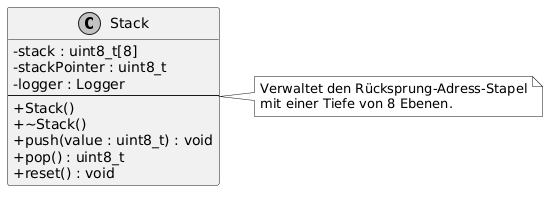
\includegraphics[width=0.9\textwidth]{UML/4.png}
\end{center}

\subsection{Negativ-Beispiel}

\textbf{Klasse: \code{PIC}} (\code{header/pic.hpp})

Die \code{PIC}-Klasse ist ein \enquote{God Object} mit mehreren Verantwortlichkeiten:

\begin{enumerate}
    \item Simulationsorchestrierung (Instruktionsausführung, Timer-Schritte)
    \item Programmmanagement (Laden, Kompilieren)
    \item Thread-sichere Zustandsabfragen für die UI (\code{getSnapshot()})
    \item Zustandsmanipulation für Debugging (\code{tryWriteRegister()}, \code{tryToggleBit()})
    \item Initialisierung aller Komponenten (Prescaler, Timer, statische Felder von \code{Instruction})
\end{enumerate}

\begin{lstlisting}[style=codeblock,language=picassocpp]
class PIC {
    ALU alu;
    Program loadedProgram;
    Register W;
    Timer timer;
    std::shared_ptr<MemoryInterface> memoryInterface;
    std::shared_ptr<Prescaler> prescaler;
    uint64_t totalSimulatedTimeUs;
    mutable std::mutex executionMutex;
    Logger logger;
    // ... 15+ öffentliche Methoden
};
\end{lstlisting}

\textbf{Lösungsweg:} Die Klasse sollte aufgeteilt werden in:

\begin{itemize}
    \item \code{PICHardware} -- hält Register, RAM, Timer (Hardware-Zustand)
    \item \code{PICSimulator} -- orchestriert Instruktionsausführung
    \item \code{PICDebugInterface} -- bietet thread-sichere Zugriffsmethoden für die UI
\end{itemize}

\begin{center}
    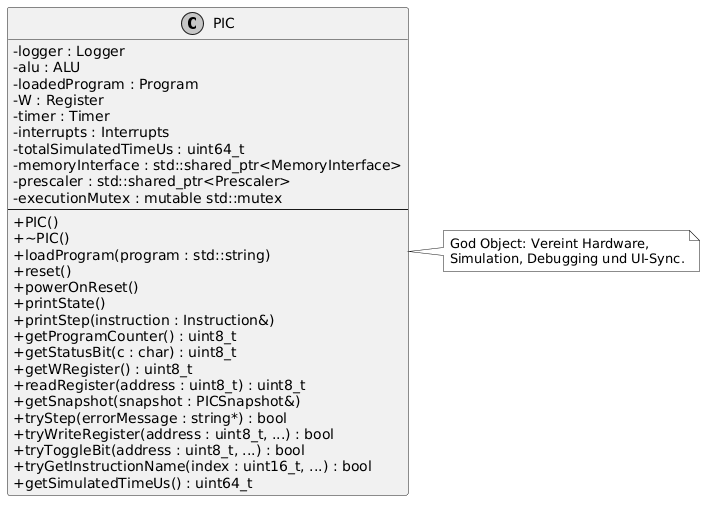
\includegraphics[width=0.9\textwidth]{UML/51.png}
\end{center}

\begin{center}
    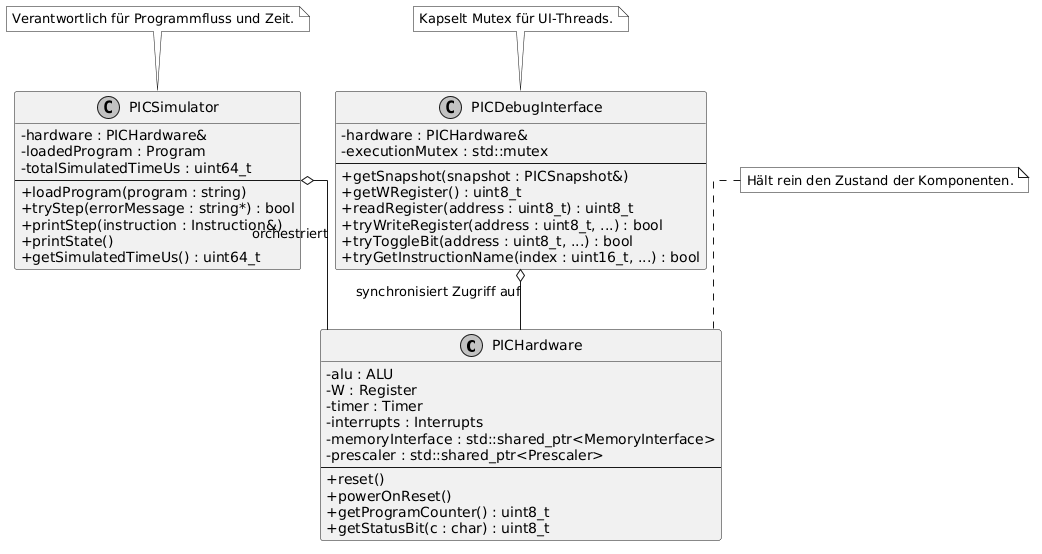
\includegraphics[width=0.9\textwidth]{UML/52.png}
\end{center}

\section{Analyse OCP}

\subsection{Positiv-Beispiel}

\textbf{Klasse: \code{Instruction}} (abstrakte Basisklasse, \code{header/instruction.hpp})

Die Klasse \code{Instruction} definiert die abstrakte Schnittstelle \code{virtual uint16_t execute() = 0}. Neue Instruktionstypen können durch Erstellen neuer Unterklassen hinzugefügt werden, ohne die Basisklasse zu modifizieren. Das Verhalten wird durch Vererbung erweitert. Beispiel: Um eine neue Instruktion hinzuzufügen, wird eine neue Klasse erstellt, die \code{Instruction} erbt und \code{execute()} implementiert.

\begin{lstlisting}[style=codeblock,language=picassocpp]
class Instruction {
    public:
        virtual uint16_t execute() = 0;   // offen für Erweiterung
        virtual std::string getName() = 0;
        virtual ~Instruction() = default;
};

class ADDWF : public Arithmetic {  // Erweiterung ohne Änderung der Basis
    public:
        uint16_t execute() override;
        std::string getName() override;
};
\end{lstlisting}

\begin{center}
    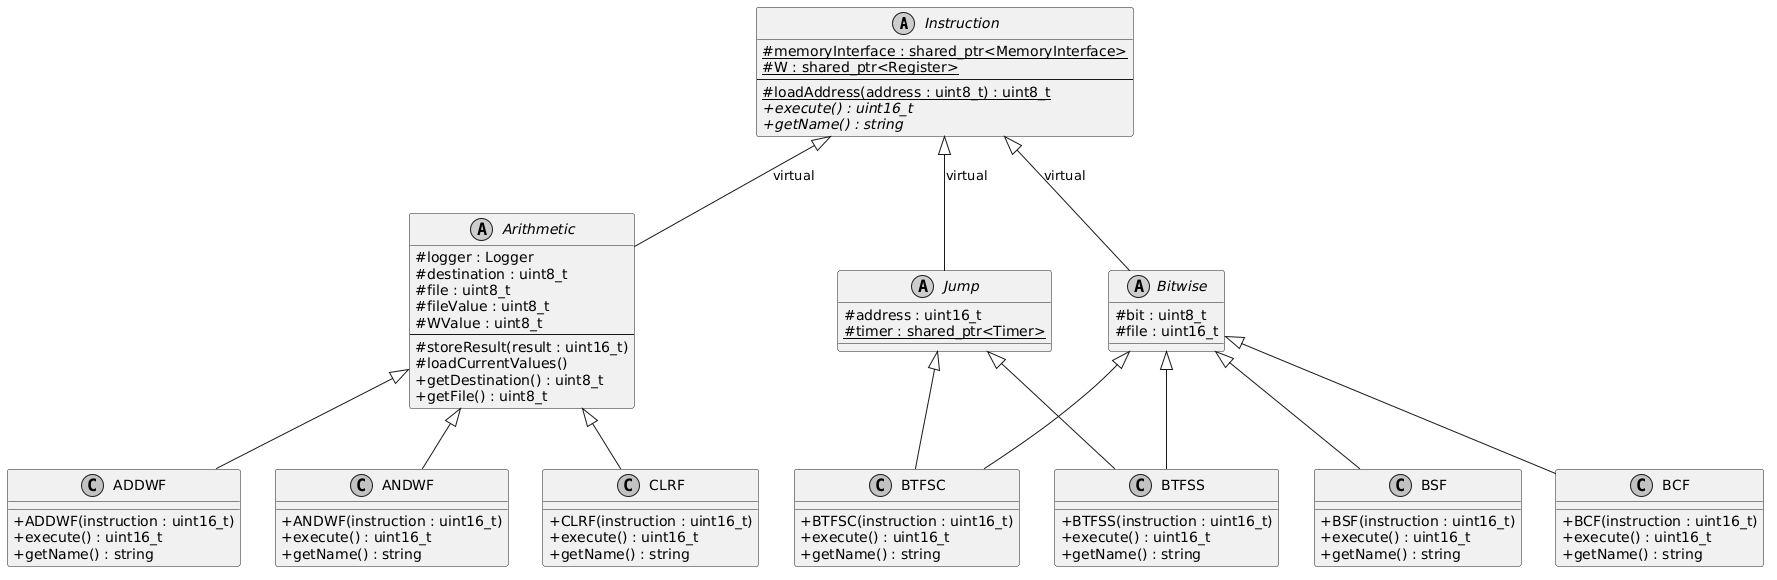
\includegraphics[height=0.5\textwidth, angle=90]{UML/6.png}
\end{center}

\subsection{Negativ-Beispiel}

\textbf{Klasse: \code{Compiler}} (\code{src/compiler.cpp})

Die Methode \code{Compiler::getInstruction()} enthält eine große Switch-Kaskade, die für jede Instruktion einen expliziten Case hat. Wenn eine neue Instruktion hinzugefügt wird, muss die Methode \code{getInstruction()} modifiziert werden -- ein klarer Verstoß gegen das Open/Closed Principle.

\begin{lstlisting}[style=codeblock,language=picassocpp]
std::unique_ptr<Instruction> Compiler::getInstruction(const uint16_t instruction) {
    switch(instruction) {
        case 0x0064: return std::make_unique<CLRWDT>(instruction);
        case 0x0009: return std::make_unique<RETFIE>(instruction);
        case 0x0008: return std::make_unique<RETURN>(instruction);
        case 0x0063: return std::make_unique<SLEEP>(instruction);
        // ... ~35 weitere Cases
    }
    // ... weitere Switch-Blöcke mit Bitmasks
}
\end{lstlisting}

\textbf{Lösung:} Ein Registry-Pattern / Factory-Map, bei der jede Instruktionsklasse sich selbst registriert:

\begin{lstlisting}[style=codeblock,language=picassocpp]
// Instruction-Factory mit Registry
using InstructionFactory = std::function<std::unique_ptr<Instruction>(uint16_t)>;
std::map<uint16_t, InstructionFactory> instructionRegistry;

// Registrierung in der jeweiligen Instruktionsklasse:
static bool registered = []() {
    instructionRegistry[0x0700] = [](uint16_t op) {
        return std::make_unique<ADDWF>(op);
    };
    return true;
}();
\end{lstlisting}


\begin{center}
    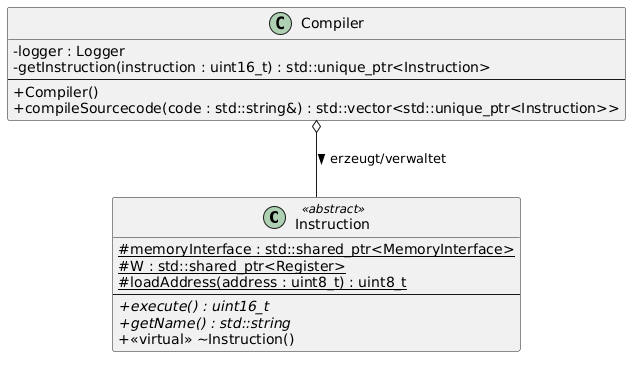
\includegraphics[width=0.9\textwidth]{UML/7.png}
\end{center}


\section{Analyse DIP}

\subsection{Positiv-Beispiel}

\textbf{Klasse: \code{ALU}} (\code{header/alu.hpp})

Die \code{ALU} hängt von der abstrakten Schnittstelle \code{Instruction} ab, nicht von konkreten Instruktionsimplementierungen. Die Methode \code{executeInstruction(Instruction&)} akzeptiert eine Referenz auf die abstrakte Basisklasse. Dadurch kann die ALU jede beliebige Instruktion ausführen, ohne konkrete Klassen zu kennen:

\begin{lstlisting}[style=codeblock,language=picassocpp]
class ALU {
    public:
        uint16_t executeInstruction(Instruction& instruction) {
            return instruction.execute();
        }
};
\end{lstlisting}

Die ALU hängt von der Abstraktion (\code{Instruction}) ab, nicht von den Details (\code{ADDWF}, \code{SUBWF}, etc.), was DIP konform ist.

\begin{center}
    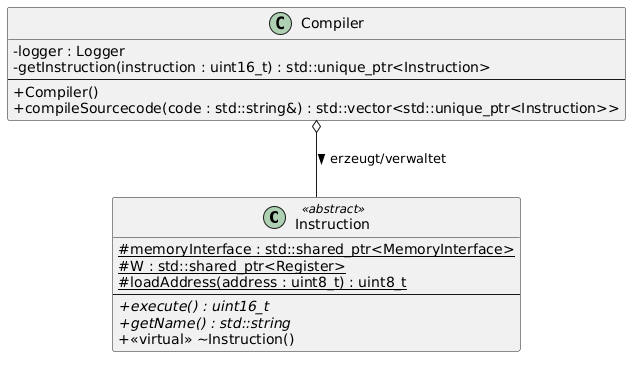
\includegraphics[width=0.9\textwidth]{UML/7.png}
\end{center}

\subsection{Negativ-Beispiel}

\textbf{Klasse: \code{PIC}}

Der PIC hängt direkt von der konkreten Implementierung des Registers ab.
Es gibt keine Abstraktionebene, gegen die Programmiert wird.
Für tests muss die konkrete Register Klasse verwendet wirden.

\begin{center}
    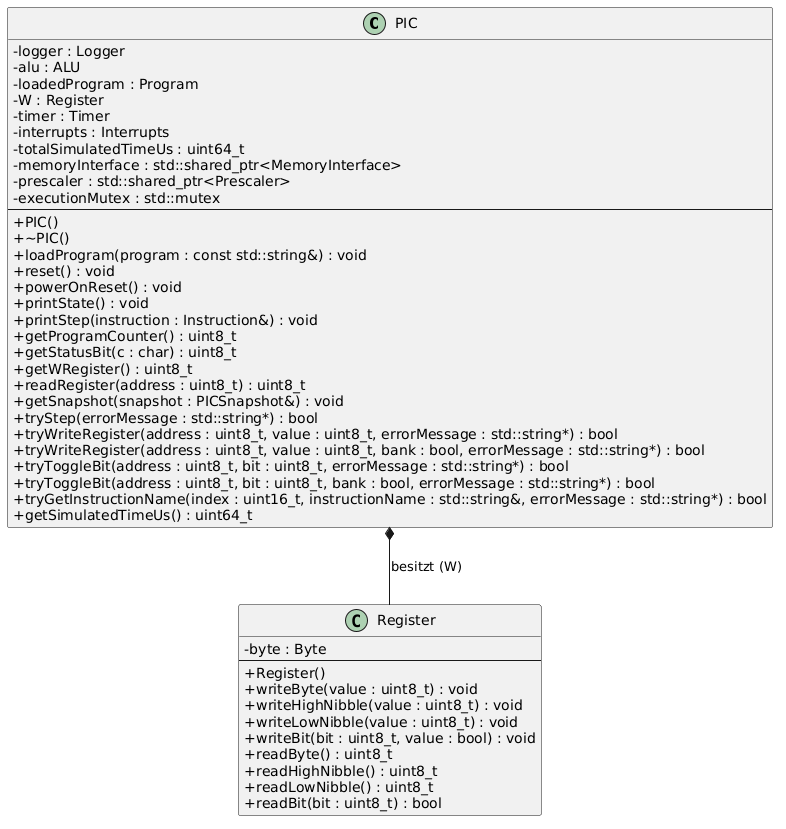
\includegraphics[width=0.9\textwidth]{UML/9.png}
\end{center}

Um dies Aufzulösen, kann eine abstrakte IRegister Klasse implementiert werden.

\begin{center}
    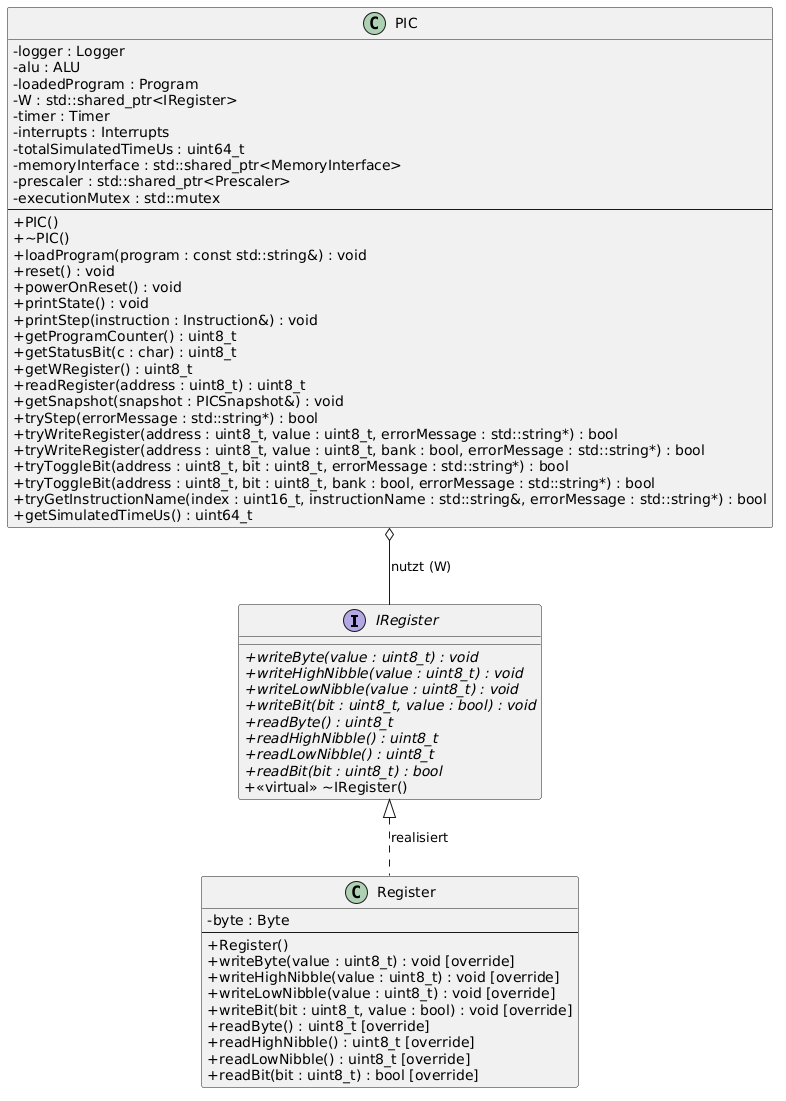
\includegraphics[width=0.9\textwidth]{UML/91.png}
\end{center}

